\chapter{基于强化学习的对抗性恶意软件生成技术架构 Adversarial Malware Generation Framework Based on Reinforcement Learning}
\section{研究的问题描述 Problem Researched Description}
近年来,随着深度学习在恶意软件检测领域的广泛应用,其高准确率与自动化能力极大提升了防御系统的智能化水平。然而,研究者相继发现深度神经网络存在严重的对抗性脆弱性——即对输入数据中微小扰动高度敏感,这些扰动在肉眼难以察觉的情况下,足以使模型输出完全错误的判断结果。这一特性被攻击者利用,催生出一种新型威胁形式:对抗性恶意软件。

In recent years, with deep learning widely adopted in malware detection, its high accuracy and automation capabilities have significantly enhanced defense systems’ intelligence. However, researchers have found that deep neural networks exhibit severe adversarial vulnerability, being extremely sensible to subtle disturbances in input data. Imperceptible to humans, these disturbances can cause models to produce entirely incorrect judgments. Attackers utilize this characteristic, catalyzing a novel threat: adversarial malware.

现有的对抗样本生成方法大多数集中于图像或文本等较为简单的数据类型。然而,在恶意软件领域,尤其是ELF文件等二进制可执行文件,扰动的设计和生成面临更多挑战。恶意软件的结构复杂且精密,任何不当的修改都可能导致文件失效或程序崩溃,因此,如何有效地生成既能绕过检测系统又能够保留恶意功能的对抗样本,是目前面临的核心问题。目前的对抗样本生成技术主要集中在静态和动态扰动上,但依然存在几个关键不足:

Current adversarial sample generation methods mostly focus on simpler data types like images or text. However, in malware realms, particularly for binary executables like ELF files, disturbance design faces greater challenges. Malware structures are so complex and precise that improper modifications may cause file failure or program crashes. Thus, how to generate adversarial samples that evade detection while ensuring malicious functionalities remains a crucial challenge. Current techniques mainly concentrate on static and dynamic disturbances but still exist critical shortcomings.

\begin{figure}[hbt]
	\centering
	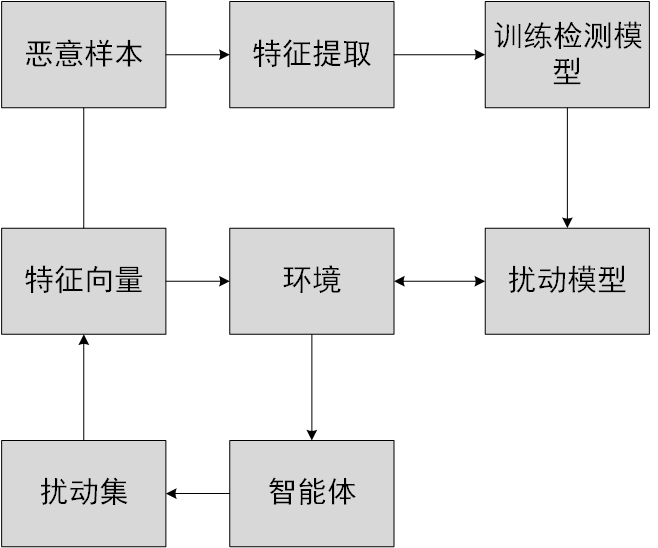
\includegraphics[width=0.75\textwidth]{figures/3.1}
	% \caption[这里的文字将会显示在 listoffigure 中]{这里的文字将会显示在正文中}
	\caption{常见对抗性恶意软件生成模型结构}\label{fig:3.1}
\end{figure}

\begin{enumerate} [label=\arabic*)] 

\item 扰动空间的局限性与复杂性 Limitations and Complexion in Disturbance Space

目前,针对对抗性恶意软件样本的生成,已有方法大多采用如字节插入、修改节区名称、篡改元数据等简单扰动手段来逃避检测系统,这类方法虽然操作便利、实现成本低,但往往缺乏结构感知与语义控制能力,其扰动维度较为单一,不能有效覆盖恶意软件在执行过程中所展现出的复杂特征。在面对复杂结构的二进制文件格式(如ELF)时,盲目扰动极易破坏文件原有逻辑或运行路径,导致样本功能失效或出现运行异常。此外,由于这类扰动方式通常在文件表层留下明显的痕迹,所生成的对抗样本容易被现代静态分析工具或启发式检测系统识别,且对抗效果往往不具备。稳定性和泛化能力。尤其在动态行为检测不断增强的背景下,如何在确保恶意功能完整的同时进行细粒度、多维度、良性扰动,成为当前对抗性样本生成研究中亟待突破的关键问题。

Existing methods for adversarial malware generation often rely on simplistic disturbances such as byte insertion, section name modification and metadata tampering, to evade detection. Although these methods are convenient to operate and are low cost, they lack structural awareness and semantic control capability. Besides, their disturbance dimensions are insufficient, which makes them hardly cover complex malware features efficiently during execution. For binary files that have intricate structure like ELF, disturbing blindly can easily disrupt file logic or execution paths, causing functional failure or abnormal behavior. Furthermore, such disturbance methods often leave obvious traces on file surfaces, making adversarial samples easily detected by modern static analysis or heuristic systems, which means the adversarial effectiveness lacks stability and generalizability. Especially in the background that dynamic behavioral detection is enhancing continuously, how to perform fine-grained, multi-dimensional and benign disturbances while ensuring functional integrity is a critical challenge to the research.

\item 扰动的合法性问题 Disturbance Legitimacy Problems

尽管当前部分对抗样本生成方法在规避恶意软件检测模型方面取得了一定成效,但其扰动策略普遍存在粗糙和随机性强的问题,常见手段包括随机字节插入、伪装节名称、修改冗余字段等浅层扰动。这类方法虽能在某些静态检测模型中绕过特征匹配机制,但缺乏对扰动合法性与语义一致性的有效控制,难以适应真实环境下多样化且复杂的检测机制。例如,随意插入的字节可能被高级检测模型识别为异常行为(如零号攻击),反而增强了恶意特征的可识别性。尤其对于依赖行为分析或异常检测的模型而言,盲目的扰动不仅无助于逃避检测,反而可能使模型学习到更具代表性的恶意特征,从而降低对抗攻击的有效性。此类“为扰动而扰动”的生成策略虽然可能在静态条件下取得短期成功,但难以保障在实际部署环境中的稳定性与隐蔽性。因此,如何构建更加结构化、具备语义感知能力的扰动策略,在不破坏原有功能的前提下提升扰动的针对性与有效性,成为当前对抗性恶意样本生成研究中的关键挑战之一。

Although current adversarial generation methods succeed in evading malware detection models, their disturbance strategies tend to be crude and highly random. Common operations include surface-level disturbances such as random byte insertion, disguised section names, and redundant byte modification. While features evade matching in static detectors, they lack effective control over disturbances legitimacy and semantic consistency, struggling against diverse real environments and detection mechanisms. For example, bytes inserted randomly may be recognized as abnormal behaviors such as zero-day attacks by advanced models, enhancing malicious feature detectability. Particularly for detection models based on behavior analysis or abnormal behavior detection, blind disturbances not only fail to evade detection but also risk teaching models more representative malicious features, reducing attack efficiency. Such strategies whose activities are only to disturb without considering effectiveness may achieve short-term static evasion but lack stability and concealment in a real deployment environment. Therefore, developing strategies that are more structural, high awareness to semantic to enhance precision and validity without losing origin functionalities is crucial.

\item 对历史扰动的依赖性缺失 Lacking Historical Disturbance Dependencies

对抗样本的生成过程本质上是一个动态决策序列,其扰动操作并非孤立发生,而是具有明显的时序依赖性——当前的扰动决策往往会受到先前扰动历史的影响。然而,现有的主流对抗样本生成方法大多将每一步扰动视为独立事件,缺乏对扰动序列内在依赖关系的建模与挖掘。这种近似于“无记忆”的策略忽略了扰动间的逻辑联系与语义上下文,导致生成的扰动序列在结构上缺乏连贯性,扰动操作之间相互脱节,甚至可能出现前后矛盾或重复无效的修改操作。这不仅降低了对抗样本的逃避能力和隐蔽性,还可能引入可疑的行为模式,反而提升被检测的风险。特别是在处理结构复杂、语义敏感的二进制恶意样本时,忽视扰动间依赖会进一步削弱攻击效果。因此,如何引入有效的时序建模机制,捕捉扰动操作之间的动态关联,从而生成更具整体性、策略性和欺骗性的扰动序列,是提升对抗样本实战能力的关键突破方向之一。

Adversarial sample generation is a dynamic decision-making sequence. Disturbance operations manifest sequential dependencies: current decisions depend on prior perturbation history, instead of isolation. However, prevalent methods treat each disturbance step as isolated, neglecting to find the inherent dependency relations. This approximately memoryless strategy ignores logical and semantic contexts between disturbances, resulting in generated sequences structural succession deficiency and disturbance operations disconnected from each other, which exhibits that some modification operations contradict with previous operations or duplicated. This result not only undermines adversarial samples’ evasion capabilities and concealment, but also potentially introduces suspicious action patterns that increase the detected rate. Especially in structurally complex, semantically sensitive malware binaries, overlooking the dependence between disturbances further reduces attack effectiveness. Therefore, introducing effective temporal modeling mechanisms to capture dynamic correlations in disturbance operations and generating more integral, strategic, deceptive disturbance sequences is a key breakthrough in enhancing adversarial sample capacities in real environments.

\item 过于关注逃逸率,忽视扰动成本与执行开销 Overemphasis on Evasion Rate and Negligence on the Cost of Execution

当前许多对抗性恶意软件生成方法普遍将“是否成功逃逸检测系统”作为主要评价指标,过度聚焦于误分类结果,而忽略了扰动过程中的多方面代价。在实际应用中,生成的对抗样本不仅需要具备较强的逃逸能力,还应兼顾扰动的实施成本与执行效率。例如,频繁或复杂的扰动操作可能导致样本体积显著增加、运行时间延长,甚至影响程序的原有功能和行为一致性,从而在实际环境中暴露风险。此外,部分策略在扰动选择上未考虑操作本身的资源消耗和可行性,导致生成的样本难以在有限计算资源下快速部署。忽视这些现实因素,往往使得对抗样本虽然能在检测模型层面绕过检查,但却在工程实际中难以落地。因此,仅以逃逸率为单一优化目标的生成策略存在明显局限,亟需引入对扰动成本与时间开销的系统性考量,以提升对抗样本的实用性与隐蔽性。

Many current adversarial malware methods mostly regard "successfully evading malware detection systems" as the primary evaluation metric, overemphasizing misclassification results while ignoring multifaceted costs of disturbance processes. However, in practical applications, not only high evasion capacities are required to adversarial samples generated, but also keeping the balance of implementation costs and execution efficiency. For example, excessive or complex disturbances significantly increase file size, prolong runtime, disrupt functionality, or affect behavioral consistency, which potentially exposes risks during execution. Furthermore, some strategies overlook resource consumption and feasibility of operations, rendering generated samples hard to deploy under constrained resources. Although ignoring these real-world factors allows samples to bypass detection models, it is a failure in engineering deployment. Therefore, the strategy that regards evasion rate as the only optimization exhibits significant limitations. It is urgent to introduce systemic consideration of disturbance costs and time to enhance sample practicality and concealment.

\end{enumerate}

本文主要的研究目的是借助强化学习和神经网络方法,构建多维度和高效的对抗样本生成方法。针对目前已有研究方法中存在的不足,本文提出以下需要解决的关键问题:

The primary objective of this research is to construct a multidimensional and efficient adversarial sample generation approach utilizing reinforcement learning and neural network methods. Addressing the shortcomings of existing methods, the following critical issues are required to resolve:

关键问题1:如何构建一个具备结构感知和语义控制能力的多维度扰动空间,以适应复杂恶意软件样本的逃逸需求?

Key Issue 1: How to construct a multidimensional disturbance space with structural awareness and semantic control capability to meet the evasion needs of complex malware samples?

关键问题2:如何提升扰动的合法性与良性,避免传统“破坏式扰动”在真实检测系统中反而暴露攻击意图?

Key Issue 2: How to enhance disturbance legitimacy and benignity, avoiding traditional "destructive disturbances" that may expose attack intentions in real detection systems?

关键问题3:如何引入扰动历史建模机制,从而生成更具连贯性和策略性的扰动序列?

Key Issue 3: How to introduce historical disturbance modeling mechanisms to generate more coherent and strategic disturbance sequences?

关键问题4:如何在对抗样本生成过程中权衡扰动有效性、功能完整性与资源开销,提升攻击样本的实际可部署性?

Key Issue 4: How to balance effectiveness, functional integrity, and resource consumption during adversarial sample generation to enhance the practical deployability of attack samples?

\section{研究的设计思路 Research Design Logic}
针对当前对抗性恶意软件样本生成方法在扰动手段粗糙、语义控制能力弱、扰动序列缺乏结构性以及忽视现实成本与可部署性等方面的不足,本文提出了一种创新的对抗样本生成框架。现有方法通常依赖简单且随机的字节插入、修改节名称等手段,缺乏对生成样本的合法性、语义一致性以及可执行性的有效控制,导致在实际环境中难以稳定有效地逃避检测。因此,本文的研究思路旨在通过系统性地优化对抗样本生成的多个关键方面,弥补这些不足。

To address current adversarial malware generation methods' limitations in coarse perturbation techniques, weak semantic control, lack of structural disturbance sequences, and neglect of practical costs and deployability, this research proposes an innovative adversarial sample generation framework. Common existing methods rely on simple, random byte insertions or section name modifications that lack effective control over sample legitimacy, semantic consistency, and executability, resulting in unstable evasion in real environments. Therefore, this research aims to solve these shortcomings by systematically optimizing multiple key aspects of adversarial sample generation.

首先,在扰动空间建模方面,本文通过引入多维度扰动技术,打破了传统方法只依赖单一扰动手段的局限,考虑到恶意软件在不同执行阶段可能展现出的多样化特征,设计了一种结构化且具有语义感知能力的扰动策略,从而避免了对文件功能的破坏,同时提高了逃避检测的难度。其次,针对扰动合法性问题,本文提出了一种基于语义一致性的扰动合法性控制方法,确保生成的对抗样本在避开检测的同时,能够维持原有的功能和行为一致性,避免了盲目扰动所带来的不稳定性。

Firstly, in the disturbance space modeling aspect, this paper introduces multidimensional disturbance techniques and breaks the limitation of traditional methods that solely rely on single disturbance methods. Since malware exhibits diverse features in different execution stages, this research designs a structural disturbance strategy with semantic awareness capacities, avoiding file functionality disruption and enhancing evasion difficulties. Secondly, targeting the disturbance legitimacy issue, a disturbance legitimacy control method based on semantic consistency is proposed to ensure adversarial samples evade detection while maintaining original functionality and behavioral consistency, avoiding instability from blind disturbances.

另外,考虑到对抗样本生成过程中的扰动序列具有明显的时序依赖性,本文通过强化学习中的PPO算法结合LSTM网络对扰动序列进行建模,从而有效捕捉扰动操作之间的动态关系,使得生成的扰动序列在整体上更加连贯、隐蔽和具备欺骗性。通过这一方法,能够优化扰动的执行顺序和策略,进一步提升对抗样本的逃避能力。

Furthermore, recognizing the obvious temporal dependency in disturbance sequences, this research employs the PPO algorithm combined with LSTM networks to model disturbance sequences, effectively capturing dynamic relationships between disturbances. This approach enhances the overall coherence, stealth, and deceptive nature of disturbance sequences, optimizing the order and strategies to further improve evasion capabilities.

最后,针对现有方法忽视扰动过程中的成本与可执行性问题,本文提出了一种新的奖励机制,除了关注检测逃逸率外,还考虑了生成过程中的资源消耗、执行时间等因素,确保生成的对抗样本不仅具备较高的攻击性,还能够在实际环境中顺利部署,避免因过于复杂的扰动操作导致样本体积膨胀、运行时间延长或功能丧失。

Lastly, addressing the neglect of disturbance costs and executability, a new reward mechanism is proposed in this research. Except for focusing on evasion rates, it considers different factors such as resource consumption and execution time, ensuring that adversarial samples are not only highly aggressive but also deployable in real environments. This prevents sample size surges, prolonged runtime, or functional loss caused by excessive disturbances.

与传统方法相比,本文具有以下几个显著优点:

\begin{enumerate} [label=\arabic*)] 

\item 结构感知的扰动空间构建:突破以往依赖静态规则或单一字节操作的扰动方式,本文在样本的结构层与语义层中引入更细粒度的操作集,设计出支持多维度、多粒度扰动的操作空间,能够更精准地定位关键行为区域并施加微扰动,从而有效提升逃避检测的灵活性和有效性。

Structurally Aware Perturbation Space Construction: Departing from previous disturbance methods relying on static rules or single-byte operations, this research introduces a finer-grained operation set at the structural and semantic layers of samples, designing an operational space supporting multidimensional and multigranular disturbances, enabling to localize key behavioral regions more precisely and apply subtle disturbances, thereby effectively enhancing the flexibility and effectiveness of evasion detection.

\item 扰动合法性与语义一致性的融合控制机制:不同于以往“只求误判、不管后果”的扰动逻辑,本文在生成过程中引入语义保持约束与合法性验证策略,确保扰动不会破坏程序原有逻辑与可执行性,从而提升对抗样本在真实系统中的稳定性与隐蔽性。

Fusion Control Mechanism for Disturbance Legitimacy and Semantic Consistency: Unlike the previous disturbance logic that only pursues misclassification regardless of consequences, this research incorporates semantic preservation constraints and legitimacy verification strategies during the generation process, which ensures that disturbances do not disrupt the original program logic and executability, enhancing the stability and concealment of adversarial samples in real systems.

\item 考虑扰动历史的序列建模机制:本文将对抗扰动过程视为一个具有时序依赖特征的策略优化任务,引入序列建模机制(如记忆单元或策略网络)来捕捉扰动操作之间的上下文关系,使生成的扰动序列更具策略性与一致性,解决了以往扰动碎片化、冗余化的问题。

Sequence Modeling Mechanism Considering Disturbance History: This research regards the adversarial disturbance process as a strategy optimization task that exhibits temporal dependency characteristics. It introduces sequence modeling mechanisms, such as memory cells or policy networks, to capture the contextual relationships between disturbance operations, which enables the sequences generated to be more strategic and consistent, addressing the previous issues that disturbances are fragmented and redundant.

\item 面向成本与开销的实用性优化目标:本文在对抗目标设计中充分考虑扰动的实施成本、样本运行效率和部署风险等实际因素,引入“轻量扰动”与“开销评估”机制,有效控制扰动规模和复杂度,使生成样本更具工程实用性,避免“虽逃逸成功却难以部署”的局限。

Optimization Objective Oriented towards Cost and Overhead Practicality: In designing the adversarial objectives, this research fully considers practical factors such as disturbance implementation cost, sample runtime efficiency, and deployment risk, introducing "lightweight perturbation" and "overhead assessment" mechanisms to effectively control the scale and complexity of disturbances. This makes the samples generated more practical for engineering deployment, thus avoiding the limitation of being evasive but hard to deploy.

\end{enumerate}

\section{研究的解决方案 Research Solutions}

针对本文3.1节中当前对抗性恶意软件样本生成方法中存在的扰动手段粗糙、语义控制能力弱、扰动序列缺乏结构性以及忽视现实成本与可部署性等问题,本文提出了一种面向实用性与隐蔽性强化的对抗样本生成框架。该框架从多个维度出发,提出了四个关键解决方案,以提高对抗样本的生成能力、逃避检测效果及实用性。

To address the issues in Section 3.1—that disturbance methods are coarse, weak semantic control, lack of structural disturbance sequences, and neglect practical costs and deployability—this paper proposes a novel adversarial sample generation framework facing practicality and concealment enhancement. This framework focuses on enhancing generation capabilities, evasion effectiveness, and practicality through 4 key solutions.

解决方案1:基于多维度的扰动空间建模

Solution 1: Disturbance Space Modeling Based on Multi-dimensions

传统的对抗样本生成方法通常采用简单的扰动方式,如字节插入、节区名称修改、冗余字段篡改等,这些方法虽然在短期内能够绕过检测,但其扰动空间较为有限,无法有效应对恶意软件复杂执行过程中的多样化特征。为此,本文提出了一种多维度扰动策略,通过精确建模多种扰动维度,从结构、指令、行为三个层面对扰动空间建模以全面覆盖恶意软件在执行过程中可能展现出的行为特征。该策略能够有效提高恶意软件样本的逃避能力和隐蔽性,同时保持样本的功能完整性。在扰动设计中,特别关注对恶意代码执行路径、控制流及其他关键结构的精确干扰,从而最大程度避免传统方法中存在的结构损坏和功能失效的问题。

Traditional adversarial sample generation methods usually employ simple disturbances, such as byte insertion, section name modification, or redundant byte modifications. While these methods may temporarily evade detection, their disturbance space is limited, failing to address the diverse features exhibited during malware execution. To address this issue, this paper proposes a multidimensional perturbation strategy. By precisely modeling various disturbance dimensions, this approach constructs a disturbance space across structural, instruction, and behavioral layers, comprehensively covering potential behavioral features during malware execution. This strategy enhances the evasion and concealment capabilities of malicious samples while preserving their functional integrity. Disturbance design particularly targets precise interference with malicious code execution paths, control flows, and other critical structures, minimizing structural damage and functional failure issues in traditional methods.

解决方案2:基于良性样本的合理化插入扰动

Solution 2: Rationalized Insertion Disturbance Based on Benign Samples

当前许多对抗样本生成方法的扰动通常依赖于随机字节插入等浅层操作,这种方式缺乏对语义合法性和扰动合理性的控制,容易导致生成样本的不稳定性或被检测到。为了解决这一问题,本文提出了一种基于良性样本的合理插入扰动方法。在这一方法中,首先通过分析良性样本的结构与行为,提取出良性样本的语义与字节结构,构建良性样本扰动库。通过对扰动进行更加结构化和语义感知的设计,保证了对抗样本在功能上的完整性和合法性,同时减少了不必要的噪声扰动。这种方法不仅能有效规避基于特征匹配的静态检测系统,还能增强对抗样本在复杂检测环境中的隐蔽性。

Current adversarial sample generation methods often rely on shallow operations, such as random byte insertion, lacking control over semantic legitimacy and disturbance rationality. This can lead samples to be unstable and to be detected easily. To overcome this disadvantage, this paper introduces a rationalized insertion disturbance method based on benign samples. By analyzing the structure and behavior of benign samples, their semantic and byte structure are extracted to build a benign sample perturbation library. This method ensures functional completeness and legitimacy of adversarial samples through more structurally and semantically aware disturbance design, reducing unnecessary noise. It not only effectively evades static detection systems based on feature matching but also enhances sample concealment in complex detection environments.

解决方案3:基于LSTM的PPO时序依赖建模

Solution 3: PPO Temporal Dependency Modeling Based on LSTM

对抗样本的生成不仅仅是每一步独立的扰动操作,而是一个具有时序依赖性的过程。现有方法通常忽略了扰动间的依赖关系,导致生成的扰动序列缺乏整体性和连贯性,从而影响逃避能力。为了解决这一问题,本文结合PPO\cite{yu2022surprising}(Proximal Policy Optimization)强化学习算法和LSTM\cite{graves2012long}(Long Short-Term Memory)模型,提出了一个联合优化的时序依赖建模方法。通过LSTM网络对扰动序列的时序关系进行建模,捕捉扰动之间的内在依赖性,PPO算法则用于优化生成策略。这一方法能够生成更具整体性、连贯性和隐蔽性的扰动序列,有效提升对抗样本的攻击性和稳定性。

Adversarial sample generation is not merely a series of independent disturbances but a process with temporal dependencies. Existing methods often overlook dependencies among different disturbances, resulting in disjointed sequences and reduced evasion capabilities. To solve this issue, this paper combines the PPO Reinforcement Learning algorithm\cite{yu2022surprising} with LSTM\cite{graves2012long} models to propose a joint optimization method for temporal dependency modeling. LSTM networks model temporal relationships in disturbance sequences, capturing intrinsic dependencies among disturbance operations, while PPO optimizes generation strategies. This method produces holistic, coherent, and stealthy disturbance sequences, enhancing adversarial sample attack effectiveness and stability.

解决方案4:基于动态奖励函数的智能体决策

Solution 4: Decision-Making Agent Based on Dynamic Reward Functions

在现有的对抗样本生成方法中,奖励函数设计往往过于简单,通常只关注样本是否成功绕过检测系统,而忽略了生成过程中的成本与效率问题。为了克服这一不足,本文提出了一种基于动态奖励函数的智能体决策机制。该机制不仅考虑逃逸成功与误分类率,还引入了扰动的资源消耗、执行效率、时间开销等因素。通过这种动态奖励机制,智能体在决策过程中能够更好地平衡攻击性与执行代价,从而生成既具备高隐蔽性,又能够快速部署的对抗样本。该方法有效提升了对抗样本的实际应用价值和部署可行性。

Existing adversarial sample generation methods often employ simplistic reward functions focused solely on whether the sample evades the detection systems, neglecting generation costs and efficiency. To address this disadvantage, this research proposes an agent-making mechanism based on dynamic reward functions. Beyond considering evasion success and misclassification rates, it incorporates factors, such as disturbance resource consumption, execution efficiency, and time costs. This dynamic reward mechanism enables agents to balance attack effectiveness with execution costs during decision-making, generating adversarial samples that are both highly stealthy and quickly deployable. This approach significantly enhances the practical application value and deployability of adversarial samples.

\section{研究的整体架构}

为了有效应对恶意软件检测系统的不断演进,提升对抗样本在真实环境下的生存能力与攻击效果,本文提出了一套系统化的对抗样本生成架构。整体设计遵循分层递进、策略引导、效果评估的原则,涵盖了数据收集、扰动策略建模、强化学习智能体训练以及奖励函数设计等关键环节,确保对抗样本能够在保证功能正确性的前提下,最大程度逃逸各类检测系统的拦截。

%\begin{enumerate} [label=(\arabic*)] 

(1) 数据收集与预处理

高质量的数据基础是对抗样本生成系统有效运行的关键前提,尤其是在针对ELF格式可执行文件的研究中,由于当前尚缺乏权威性、标准化的公开数据集,这一问题尤为突出。为弥补该空白,本文自主构建了一个覆盖面广、结构多样的ELF样本集,涵盖恶意样本与正常样本两个维度,确保后续模型训练与扰动策略评估具有良好的实验基础与推广能力。

在恶意样本采集方面,本文主要从VirusShare\cite{VirusShare}、Maltrieve等知名的开源恶意软件平台中筛选并下载经过多重验证的x86架构下的ELF格式恶意样本。样本类型涵盖多种常见攻击形式,包括蠕虫传播程序、加密货币挖矿程序、远程控制型后门程序、DDoS工具及嵌入式木马等,具有较强的代表性与研究价值。为进一步提升样本质量,本文对收集到的样本进行了格式校验、哈希去重、恶意行为标签确认等预处理操作,确保样本集的真实性与一致性。在正常样本采集方面,本文基于QEMU虚拟化技术搭建了多个目标运行环境,主要包括基于Raspbian和OpenWrt的ARM架构嵌入式系统,以及基于Ubuntu的x86系统环境,从中提取了系统默认运行的合法ELF程序,如系统工具、守护进程、配置脚本等。这些样本在功能完备、结构规范的同时,能够覆盖多种开发工具链和构建方式,进一步增强了正常样本集的多样性与代表性。

为了确保数据集的质量与准确性,本文在完成初步样本收集后,针对所有获取的ELF格式可执行文件样本均引入了VirusTotal\cite{VirusTotal}平台的复审机制,以增强样本标注的权威性与恶意性确认的可信度。具体而言,首先对每个样本执行SHA-256等哈希指纹提取操作,构建唯一标识,剔除重复或冗余的样本项,确保样本集的去重和纯净;随后将样本上传至VirusTotal平台,通过其集成的多引擎病毒扫描系统(涵盖Kaspersky、Avast、BitDefender、ESET等多个主流安全厂商)进行全面检测。

在扫描过程中,本文重点关注引擎返回的检测标签、恶意评分(malicious score)、行为分析结果以及YARA规则匹配情况等关键信息,构建每个样本对应的检测报告元数据集,用于后续的分析、训练与评估。同时,对于存在标注不一致或引擎分歧较大的边界样本,通过引入手动复审或多轮投票方式进一步判断其可信分类,保证数据标注的一致性和准确性。
此外,扫描报告中所提取的信息(如API调用特征、连接行为、时间戳等)也为后续的扰动操作设计与对抗样本生成提供了参考依据,帮助理解当前主流检测机制所侧重的关键特征,从而指导扰动策略选择。

(2)扰动策略构建

针对现代恶意软件检测系统在静态、动态以及行为特征等多维度的集成分析机制,本文提出了一种具有分层次特征的组合式扰动策略,旨在从结构信息、指令序列和动态行为三个层面入手,打破传统特征提取链条,从而提升对抗样本的隐蔽性与鲁棒性。在现有检测系统中,往往通过固定规则或训练模型提取静态特征(如节结构、函数调用图、符号信息)、指令级特征(如n-gram、CFG路径)以及动态行为(如系统调用序列、内存行为等),因此,设计能够有效扰乱这些检测路径的扰动机制对于生成高质量对抗样本具有重要意义。

在结构扰动方面,本文主要采用插入式结构变换策略,该策略具有较好的通用性和对原程序功能的非破坏性。具体方法包括在ELF二进制文件中插入伪造节(section)和无效段(segment),例如通过LIEF库\cite{LIEF2025}动态创建.fake、.dummy\_code等节,且这些节不参与程序逻辑流程,仅作为混淆成分存在;同时对ELF头部(ELF Header)、程序头表(Program Header Table)及节区头表(Section Header Table)进行轻量修改,如调整节表顺序、伪造入口点地址、添加重定位信息等,使得静态分析工具在解析时产生偏差。此外,还包括对程序进行壳处理(packing)和脱壳(unpacking)操作,通过UPX等压缩工具实现结构扰动,并结合反壳策略恢复执行能力,从而扰乱基于字节签名和结构模式匹配的检测系统。

\begin{figure}[hbt]
	\centering
	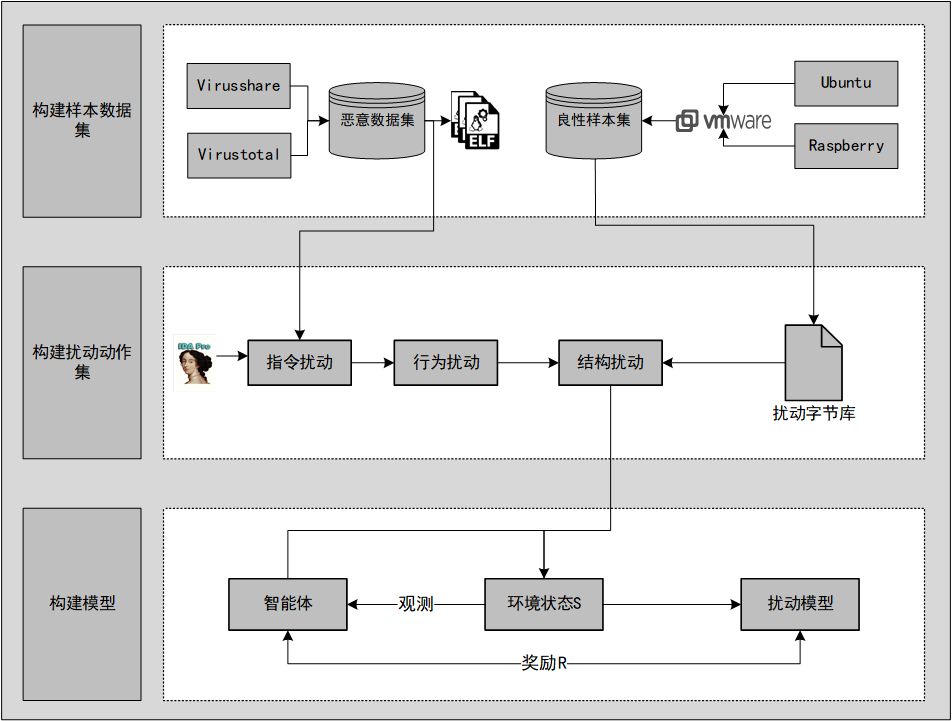
\includegraphics[width=0.75\textwidth]{figures/3.2}
	% \caption[这里的文字将会显示在 listoffigure 中]{这里的文字将会显示在正文中}
	\caption{基于强化学习的对抗性样本生成方法框架}\label{fig:3.2}
\end{figure}


在指令层面,本文通过结合IDA Pro、radare2等反汇编工具,对原始二进制样本进行静态反汇编与控制流图提取,进而实现对指令的扰动式重写。首先,在保证程序语义不变的前提下,使用等价指令替换技术,例如用xor eax, eax替换mov eax, 0,或使用冗余的加法/减法指令链完成简单赋值,扰乱检测模型对常规语义的理解;其次,利用寄存器交换策略(如将eax换为ebx等)打破寄存器使用模式,同时修改跳转指令逻辑,在跳转目标不变的情况下引入间接跳转、中间跳板、无效跳转等手段,以此增加CFG的复杂度,干扰以控制流为特征的静态图分析器。在指令组合上,本文还引入了无效填充操作,如NOP滑块(NOP sled)与空函数调用序列,进一步加大模型提取有效语义片段的难度。

针对动态分析系统的行为建模特性,本文设计了一套动态执行扰动机制,旨在规避基于沙箱技术的行为检测模型。该机制通过修改程序实际入口点(Entry Point),优先执行伪造行为逻辑,再逐步过渡到真实恶意载荷执行,从而在短时间行为采集窗口中有效延迟真实行为暴露。常用策略包括添加自循环逻辑(例如构造伪循环结构)、空跳转路径(无逻辑变化但执行时间延长)以及插入系统级延迟调用,如sleep()、nanosleep()等API,来阻断沙箱的行为提取流程。此外,还可嵌入虚拟环境检测语句(如CPUID指令、MAC地址识别等),使得样本在虚拟分析平台上呈现不同行为路径,进一步规避检测。结合动态段的无效控制流插入,本文的扰动策略在沙箱动态行为分析阶段展现出良好的逃避性能。

(3)奖励函数策略优化

在本研究中,强化学习(RL)模型的奖励函数设计是生成对抗性恶意软件样本的核心要素之一。为了使智能体能够有效地避开恶意软件检测系统,并生成具有足够复杂性的对抗样本,本文提出了一种综合考虑检测逃逸、样本多样性和生成复杂度的奖励函数。奖励函数的优化与构建直接决定了智能体在训练过程中的学习效果和最终生成的恶意样本的质量。

首先,奖励函数的主要目标是鼓励智能体生成能够避开现有检测系统的恶意样本。因此,奖励函数首先根据样本是否能够逃避检测来给予奖励。当智能体生成的样本未被恶意软件检测模型判定为恶意时,智能体将获得一个正向奖励,反之则给予负向奖励。这个反馈机制可以引导智能体在生成过程中不断优化策略,以提高恶意样本的逃逸能力。

其次,样本的多样性也是奖励函数中一个重要的考虑因素。在对抗性样本生成过程中,若智能体能够通过修改程序的控制流、修改函数调用顺序、插入随机字符串等方式增加样本的多样性,将会获得相应的奖励。通过这种方式,奖励函数促进了恶意样本的多样化,避免了模型生成过于单一或重复的样本,从而提高了生成样本的泛化能力。

最后,为了避免智能体在生成样本时产生过于复杂或不稳定的结果,本文在奖励函数中引入了对样本复杂度的惩罚机制。当生成的恶意样本过于复杂(例如,通过过多的控制流操作或冗长的代码片段),智能体将受到一定的惩罚。这一策略帮助智能体在保证逃逸能力的同时,生成更加稳定和有效的样本,从而提高生成的样本的实际应用价值。

为了使奖励函数更加灵活和适应不同训练阶段,本文还采用了动态调整策略。在训练的初期,智能体主要依赖于探索奖励,通过多样化的变异操作来探索不同的恶意样本类型。随着训练的进展,探索奖励逐步减少,智能体将更多地依赖于利用已知的优秀策略,以生成更加高效和复杂的恶意样本。这种动态调整机制确保了智能体能够在探索和利用之间找到平衡,并逐步提升生成样本的质量。

(4)强化学习模型构建与训练

在前述模型架构中,本文设计了强化学习的智能体,旨在通过持续优化恶意软件样本生成过程以规避检测。为了提升智能体的决策能力和生成样本的多样性,本文采用了LSTM和PPO相结合的强化学习模型。

首先,LSTM被集成到智能体的策略网络中,以便捕捉生成过程中的长期依赖关系。恶意软件样本的生成过程通常是序列化的,每一步生成的行为不仅依赖于当前的输入,还受到之前生成步骤的影响。LSTM作为一种循环神经网络,能够有效存储并利用这些历史信息,从而增强模型在生成恶意样本时的准确性和灵活性。通过这种方式,智能体能够在执行每一个生成操作时考虑到先前的生成状态,进而做出更加合理的决策,减少生成结果的不一致性。

在此基础上,PPO强化学习算法被用来进一步优化策略的更新过程。PPO作为一种近端策略优化方法,利用了较为稳定的策略更新机制,有效避免了策略的剧烈波动。通过控制每次策略更新的幅度,PPO能够保证智能体在不断尝试和学习的过程中,既能够快速提高生成效果,又能避免由于过度优化而导致的不稳定。PPO通过对策略网络的不断优化,使得智能体能够逐步学会如何在恶意软件生成过程中最大化逃避检测系统的概率,从而提高生成样本的攻击性和隐蔽性。

在训练过程中,智能体每生成一个恶意软件样本,就会根据检测模型给出的评分作为奖励反馈给智能体。这些奖励信号作为训练的动力,推动策略网络的优化。为了增强训练的稳定性,本文采用了经验回放机制和奖励归一化技术。这些方法使得智能体在学习过程中能够更加高效地利用过去的经验,同时避免由于奖励过大或过小导致学习不平衡的情况。

通过这种结合LSTM和PPO的方法,智能体能够在恶意软件生成任务中不断优化其生成策略。最终,训练完成的模型能够生成具有高度复杂性和隐蔽性的恶意软件样本,这些样本能够有效地避开现有的恶意软件检测系统,提升了对抗性样本生成的能力。

%\end{enumerate}
\section{本章小结}

本章首先介绍了当前恶意软件检测领域中面临的挑战,特别是在应对新型对抗性样本时,传统的检测方法往往无法有效识别。通过分析现有技术的不足之处,发现许多传统方法所存在的问题。针对这些问题,本章提出了对应的解决方案。接下来,本章详细介绍了这一解决方案的设计思路。通过强化学习算法,代理能够在训练环境中与检测模型互动,学习如何生成绕过检测的恶意样本。这一过程通过奖励机制引导代理生成具有高隐蔽性和变异性的样本,从而提升恶意软件的复杂度和变化性,使得现有的检测方法更难识别。最后,本章描述了整个系统的整体架构设计。该架构包括数据收集与处理、扰动策略构建、奖励函数策略优化与强化学习模型构建与训练四个部分以实现本文的研究目标,完成对抗样本的生成。

